\chapter{Sistemi lineari tempo-invarianti}
Un sistema fisico di elaborazione di un segnale può essere visto come una black box che riceve in ingresso uno o più segnali e restituisce in uscita uno o più segnali, in generale alterati in modo diverso a diverse frequenze.
\begin{figure}[h]\centering
\begin{tikzpicture}[node distance=2cm]
\node [block] (system) at (0,0) {S};
\node [left of=system](input) {$s(t)$};
\node [right of=system] (output) {$r(t)$};
\draw [-latex] (input) -- (system);
\draw [-latex] (system) -- (output);
\end{tikzpicture}
\end{figure}

\section{Classificazione dei sistemi}
Si classificano i sistemi per le seguenti proprietà:

\textbf{Memoria}: Un sistema \emph{privo di memoria} ha uscita $r(t)=f[s(t)]$ che dipende solo dal valore di s in $t$ altrimenti è \emph{dotato di memoria}.

\textbf{Causalità}: Un sistema è causale se l'uscita $r(t_0)$ dipende dai valori assunti da $s(t)$ per $t\leq t_0$, \emph{anti-causale}, l'uscita è influenzata da valori futuri dell'ingresso.

\textbf{Tempo invarianza}: Un sistema tempo-invariante presenta lo stesso segnale di uscita in risposta ad un ingresso ritardato
\[\begin{split}s(t)&\to r(t)\\s(t-\tau)&\to r(t-\tau)\end{split}\]

\textbf{Invertibilità}: Un sistema inverso può riportare la risposta $r(t)$ di un sistema al segnale originale $s(t)$
\begin{figure}[!ht]
	\begin{center}\begin{tikzpicture}[node distance=2cm]
		\node [block,node distance=3cm] (system) at (0,0) {S};
		\node [left of=system](input) {$s(t)$};
		\node [block, right of=system, node distance=3cm] (inverse) {$S^{-1}$};
		\node [right of=inverse] (output) {$s(t)$};
		\draw [-latex] (input) -- (system);
		\draw [-latex] (system) -- (inverse) node[pos=.5,below] {$r(t)$};
		\draw [-latex] (inverse) -- (output);
		\end{tikzpicture}
	\end{center}
\end{figure}

\textbf{Linearità} Un sistema per cui vale il principio di sovrapposizione degli effetti, per cui dati $s_1(t)\to r_1(t)$ e $s_2(t)\to r_2(t)$, alla combinazione lineare degli effetti corrisponde la combinazione lineare delle uscite \[a\cdot s_1(t)+ b\cdot  s_2(t)\to a\cdot r_1(t)+b\cdot r_2(t)\]

\textbf{Stabilità} Un sistema \textsc{BIBO}-stabile ha una uscita limitata in risposta ad un ingresso limitato
\[\abs{s(t)}<\infty\ \exists R_\text{max}<\infty\ni'\forall t\abs{r(t)}<R_\text{max}\]

\section{Risposta all'impulso}
In un sistema lineare vale il principio di sovrapposizione degli effetti. Qualunque segnale in ingresso  si può rappresentare come somma di infiniti impulsi $s(t)=s(t)\ast\delta(t)=\intinf{s(\tau)\delta(t-\tau)}{\tau}$

Si può calcolare la risposta del sistema a qualunque ingresso $s(t)$ conoscendo la risposta all'impulso $\delta(t)\to h(t)$ o più in generale in funzione di $t$ e da un istante iniziale $\tau$: $\delta(t-\tau)\to h(t,\tau)$ come
\[r(t)=\intinf{s(\tau)h(t,\tau)}{\tau}\]

\begin{figure}[!ht]
	\begin{center}\begin{tikzpicture}[node distance=2cm]
		\node [block] (system) at (0,0) {S};
		\node [left of=system](input) {$\delta(t-\tau)$};
		\node [right of=system] (output) {$h(t,\tau)$};
		\draw [-latex] (input) -- (system);
		\draw [-latex] (system) -- (output);
		\end{tikzpicture}
	\end{center}
\end{figure}

Se il sistema è \textsc{LTI} lineare tempo invariante $h(t,\tau)=h(t-\tau)$, per cui si ha il risultato notevole che qualunque risposta del sistema si ottiene come convoluzione del segnale di ingresso con la risposta all'impulso del sistema
\begin{equation}
r(t)=\intinf{s(\tau)h(t-\tau)}{\tau}=s(t)\ast h(t)
\end{equation}

\section{Sistemi Lineari Tempo Invarianti}
Per i sistemi LTI la risposta in frequenza del sistema ha trasformata di Fourier
\begin{equation}
\begin{split}r(t)&=s(t)\ast h(t)\\R(f)&=S(f)\cdot H(f)\end{split}
\end{equation}

Si tratta di sistemi privi di memoria per cui l'uscita dipende solo dal segnale in ingresso in $t$, $r(t)=f[s(t)]$, il che implica una risposta all'impulso $h(t)=k$ costante.

Sono sistemi causali in cui $r(t_0)$ dipende dai valori $s(t)$ per $t<t_0$.

La stabilità BIBO per sistemi LTI implica l'assoluta integrabilità della risposta all'impulso (rispetta le condizioni di Dirichlet)
\[ \text{LTI BIBO}\iff \intinf{\abs{h(t)}}{t}<\infty \]
\`{E} possibile ottenere il sistema inverso che restituisca il segnale in ingresso, che abbia una risposta all'impulso tale che $h(t)\ast g(t)=\delta(t)$ ovvero
\[H(f)\cdot G(f)=1 \qquad G(f)=\frac{1}{H(f)}\]

Un sistema LTI con in ingresso un segnale di energia ha in uscita un segnale di energia
\[ E_s=\intinf{\abs{S(f)}^2}{f} \qquad E_r=\intinf{\abs{S(f)}^2 \abs{H(f)}^2}{f} \]
\begin{nota}Proprietà importante dei sistemi LTI per i filtri lineari in cui interessa dimensionare soprattutto la banda passante e l'energia / densità spettrale di energia.\end{nota}

\section{Filtri ideali}
\subsection{Filtro passa basso ideale}\index{filtro!passa basso}
Il filtro passa basso ideale elimina tutte le frequenze non comprese nella banda passante $f\in[-B,B]$.
\begin{figure}[!ht]
\centering\begin{tikzpicture}[scale=.8]
\begin{axis}[axis lines=middle,no markers,enlargelimits,xscale=2,xtick={-.5,0,.5},xticklabels={$-B$,$0$,$B$},ytick={0,1},xlabel=$f$,ylabel=$H_\text{LP}(f)$]
\addplot [very thick,samples=100,domain=-1:1]  {abs(x)<.5?1:0};
\addplot [dashed,samples=11,domain=-1:1]  {abs(x)<.5?1:0};
\end{axis}
\end{tikzpicture}
\end{figure}
\begin{equation}
H_\text{LP}(f)=\rect{\frac{f}{2B}}\qquad h_\text{LP}(t)=2B\sinc{2 B t}
\end{equation}\label{eq:filtro_passa_basso_ideale}

\`{E} ideale perché per filtrare tutte le frequenze al di fuori dell'intervallo bisognerebbe conoscere il segnale nel tempo anche per valori futuri (filtro anti-causale non fisicamente realizzabile).
\begin{nota}Il filtro passa basso viene applicato sempre prima di altri filtri amplificatori per attenuare il rumore non desiderato che ha energia a tutte le frequenze.\end{nota}

\subsection{Filtro passa alto ideale}\index{filtro!passa alto}
Il filtro passa alto ideale fa passare tutte le frequenze al di fuori dell'intervallo $[-B,B]$. \`{E} ideale perché non è possibile avere una risposta all'impulso, che ha energia finita, che abbia energia infinita. Il filtro reale si attenua alle più alte frequenze.
\begin{figure}[!ht]
	\centering\begin{tikzpicture}[scale=.8]
	\begin{axis}[axis lines=middle,no markers,enlargelimits,xscale=2,xtick={-.5,0,.5},xticklabels={$-B$,$0$,$B$},ytick={0,1},xlabel=$f$,ylabel=$H_\text{LP}(f)$]
	\addplot [very thick,samples=100,domain=-1.5:1.5]  {abs(x)>.5?1:0};
	\addplot [dashed,samples=11,domain=-1:1] {abs(x)>.5?1:0};
	\addplot [dashed,samples=11,domain=-2:-1] {x+2};
	\addplot [dashed,samples=11,domain=1:2] {-x+2};
	\end{axis}
	\end{tikzpicture}
\end{figure}
\begin{equation}
H_\text{HP}(f)=1-H_\text{LP}(f)\qquad h_\text{HP}(t)=\delta(t)-2B\sinc(2 B t)
\end{equation}

\subsection{Filtro passa banda ideale}\index{filtro!passa banda}
Il filtro passa banda ideale fa passare le frequenze attorno a $f_0$ tra $f_L$ e $f_H$ e attorno a $-f_0$ tra $-f_H$ e $-f_L$ con banda $B=f_H-f_L$.

\begin{figure}[!ht]
	\centering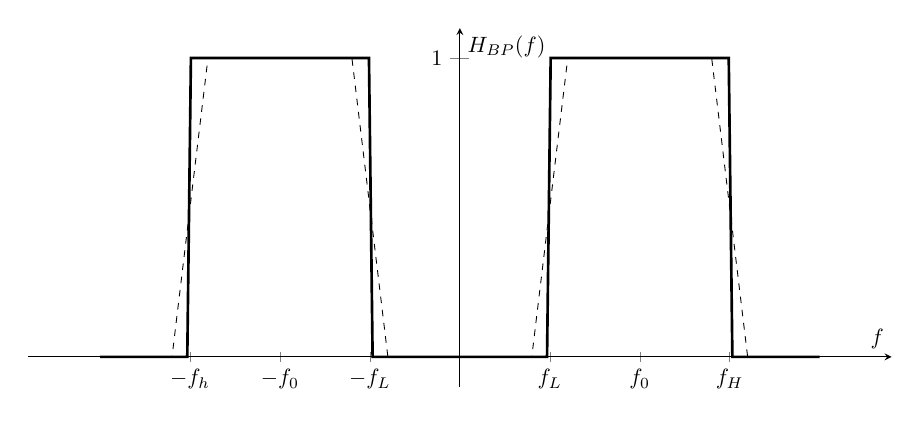
\begin{tikzpicture}[scale=.8]
	\begin{axis}[axis lines=middle,no markers,enlargelimits,xscale=2,xtick={-1.5,-1,-.5,0,.5,1,1.5},xticklabels={$-f_h$,$-f_0$,$-f_L$,$0$,$f_L$,$f_0$,$f_H$},ytick={0,1},xlabel=$f$,ylabel=$H_\text{BP}(f)$]
	\addplot [very thick,samples=100,domain=-2:0]  {abs(x+1)<.5?1:0};
	\addplot [very thick,samples=100,domain=0:2]  {abs(x-1)<.5?1:0};
	\addplot [dashed,samples=11,domain=-2:0]  {abs(x+1)<.5?1:0};
	\addplot [dashed,samples=11,domain=0:2]  {abs(x-1)<.5?1:0};
	\end{axis}
	\end{tikzpicture}
\end{figure}

Si definisce il \textsc{fattore di qualità} $Q=\frac{f_0}{B}$, che risulta tanto migliore quanto più è stretta la banda attorno alla frequenza $f_0$.
\begin{equation}H_\text{BP}(f)=\rect{\frac{f-f_0}{B}}+\rect{\frac{f+f_0}{B}}\end{equation}
\[h_\text{BP}(t)=B\sinc{B t}\e{\imath 2\pi f_0 t}+B\sinc{B t}\e{-\imath 2\pi f_0 t}=2 B\sinc{B t}\cos{2\pi f_0 t}\]

\begin{figure}[!ht]
\centering\begin{tikzpicture}
\begin{axis}[axis lines=middle,no markers,enlargelimits,xscale=2,xtick={-9.424,-6.283,-3.141,0,3.141,6.283,9.424},ytick={0,2},xticklabels={$-\frac{3}{B}$,$-\frac{2}{B}$,$-\frac{1}{B}$,$0$,$\frac{1}{B}$,$\frac{2}{B}$,$\frac{3}{B}$},yticklabels={$0$,$2B$},ylabel={$h_\text{BP}(t)$}]
\addplot [thick,domain=-3.5*pi:3.5*pi,samples=300] { (2*sin(x)/x)*cos(8*x) };
\addplot [dashed,domain=-3.5*pi:3.5*pi,samples=100] { (2*sin(x)/x) };
\end{axis}\end{tikzpicture}\caption{Filtro passa banda ideale}
\end{figure}

\begin{esempio}
Esempio di filtro passa basso realizzato con circuito \textsc{RC}.
\begin{figure*}[h]
\centering\begin{circuitikz}
\draw (0,0)	to[open,v^>=${V_i(t)}$] (0,3)
	to[R, l=${R}$, *-] (3,3)
	to[C, l=${C}$,i>_=${i(t)}$] (3,0) to[short,-*] (0,0)
	(3,0) -- (4,0) to[open,v>=${V_u(t)}$, *-*] (4,3) -- (3,3)
	(1.5,1.5) node[scale=3]{$\circlearrowright$}
	(1.5,1.5) node{$i(t)$};
\end{circuitikz}\caption{Filtro passa basso realizzato con circuito RC}
\end{figure*}
La tensione sul condensatore $v_c$ pari alla tensione di uscita $v_u$
\[v_u(t)=\frac{q(t)}{C}\]
\[\deriv{v_u(t)}{t}=\frac{1}{C}i(t)\]
L'equazione differenziale che descrive l'andamento delle tensioni
\[v_i(t)=R i(t)+ v_u(t)=R C \deriv{v_u(t)}{t} + v_u(t)\]
Trasformata secondo Fourier
\[V_i(f)=R C \imath 2\pi f_o V_u(f) + V_u(f)\]
Funzione di trasferimento ingresso-uscita
\[H(f)=\frac{V_i(f)}{V_u(f)}=\frac{1}{1+\imath 2\pi f R C}\]
dove $f_T=\frac{1}{2\pi R C}$ rappresenta la frequenza di taglio.
\begin{figure}[!ht]
\centering\begin{tikzpicture}[scale=.8]
\begin{axis}[axis lines=middle,no markers,enlargelimits,xscale=1.5,xtick={.159},xticklabels={$f_T$},ytick={0,1},xlabel=$f$,ylabel=$\abs{H(f)}$]
\addplot [very thick,samples=200,domain=-1:1]  {1/(sqrt(1+(2*pi*x)^2))};
\addplot [dashed] coordinates {(-.159,.707)(.159,.707)(.159,0)};
\end{axis}
\end{tikzpicture}
\caption{Modulo della funzione di trasferimento}
\end{figure}

La risposta in ampiezza espressa in decibel, come confronto tra potenze relative ad un riferimento
\[\abs{H(f)}_\text{dB}=10\Log\frac{\abs{H(f)}^2}{\abs{H(f_0)}^2}\]
si calcola sulla potenza del segnale, ovvero alla sua risposta in ampiezza al quadrato
\[\abs{H(f)}^2=\frac{1}{1+(2\pi f R C)^2}\]
calcolata rispetto al riferimento $f_0=0$ per cui $\abs{H(f_0)}^2=1$

Alla frequenza di taglio $f_T=\frac{1}{2\pi R C}$ si dimezza il modulo quadro ovvero si ha una attenuazione pari a 
\[\abs{H\left(f_T\right)}_\text{dB}=10\Log\frac{1}{2}=-3\text{dB}\]

\begin{figure}[!ht]
	\centering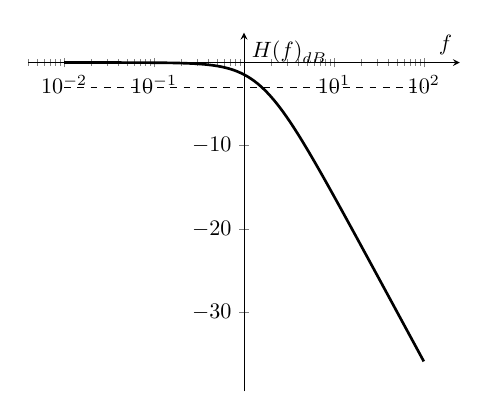
\begin{tikzpicture}[scale=.8]
	\begin{axis}[xmode=log,axis lines=middle,no markers,enlargelimits,xlabel=$f$,ylabel=$\abs{H(f)}_\text{dB}$]
	\addplot [very thick,samples=200,domain=.01:100]  {-10*log10( 1+(2*pi*x*.1)^2)};
	\addplot [dashed] coordinates{(.01,-3)(100,-3)};
	\end{axis}
	\end{tikzpicture}
	\caption{Modulo in decibel della funzione di trasferimento}
\end{figure}
\end{esempio}

\section{Autocorrelazione per segnali ad energia finita}
Si definisce per segnali ad energia finita la funzione \keyword[segnale!autocorrelazione]{autocorrelazione}, grandezza che indica quanto un segnale $x(t)$ sia simile ad una sua replica ritardata di un tempo $\tau$
\begin{equation}R_x(\tau)=\intinf{x(t)\conj{x}(t-\tau)}{t}=x(\tau)\ast \conj{x}(-\tau)\end{equation}
La trasformata di Fourier del prodotto di convoluzione \footnote{essendo $x(-t)\overset{\Fourier}{\to}X(-f)$ mentre $\conj{x}(t)\overset{\Fourier}{\to}\conj{X}(-f) \implies \conj{x}(-t)\overset{\Fourier}{\to}\conj{X}(f)$
}
\[x(\tau)\ast \conj{x}(-\tau)\overset{\Fourier}{\to}X(f)\conj{X}(f)\]

La funzione di autocorrelazione è anche l'antitrasformata di Fourier dello spettro di energia del segnale
\begin{equation}
R_x(\tau)=\intinf{\abs{X(f)}^2\e{\imath 2\pi f\tau}}{\tau}
\end{equation}

\textbf{Proprietà}
\begin{enumerate}
\item La funzione di autocorrelazione calcolata per $\tau=0$ coincide con l'energia del segnale
\[R_x(0)=\intinf{x^2(t)}{t}=E_x\]
\item La funzione di autocorrelazione è una funzione pari
\[R_x(\tau)=R_\conj{x}(-\tau)\]
\emph{Dim.} Facilmente dimostrabile in frequenza 
\[\begin{split}R_x(\tau)&=\intinf{\abs{X(f)}^2\e{\imath 2\pi f\tau}}{\tau}\\
R_x(-\tau)&=\intinf{\abs{X(f)}^2\e{-\imath 2\pi f\tau}}{\tau}\\
R_\conj{x}(-\tau)&=\intinf{\abs{X(f)}^2\e{\imath 2\pi f\tau}}{\tau}\end{split}\]
\item Il massimo della funzione di autocorrelazione si ha per $\tau=0$
\[\abs{R_x(\tau)}\leq R_x(0)\]
\emph{Dim.}
\[\begin{split}\abs{R_x(\tau)}^2=\abs{\intinf{x(t)x(t-\tau)}{t}}^2&\leq\intinf{\abs{x(t)}^2\abs{x(t-\tau)}^2}{t}\leq\\\leq&\intinf{\abs{x(t)}^2}{t}\cdot\intinf{\abs{x(t-\tau)}^2}{t}=R_x^2(0)\end{split}\]
\end{enumerate}

\section{Cross correlazione}
Si definisce la \keyword[segnali!cross-correlazione]{cross-correlazione} tra due segnali $x(t)$ e $y(t)$ la misura della somiglianza tra due segnali tra cui intercorre un ritardo di un tempo $\tau$
\begin{equation}R_{xy}(\tau)=\intinf{x(t)\conj{y}(t-\tau)}{t}=x(\tau)\ast \conj{y}(-\tau)\end{equation}
\begin{equation}R_{yx}(\tau)=\intinf{y(t)\conj{x}(t-\tau)}{t}=y(\tau)\ast \conj{x}(-\tau)\end{equation}
Si può dimostrare che \[R_{xy}(\tau)=R_\conj{yx}(-\tau)\] infatti se $R_{yx}(\tau)=y(\tau)\ast \conj{x}(-\tau)\implies R_\conj{yx}(\tau)=\conj{y}(\tau)\ast x(-\tau)\implies
R_\conj{yx}(-\tau)=\conj{y}(-\tau)\ast x(\tau)=R_{xy}$.

Due segnali si dicono \keyword[segnali!ortogonali]{ortogonali} se sono incorrelati qualunque sia il ritardo $\tau$ \[R_{xy}(\tau)=0\;\forall\tau\]

\section{Autocorrelazione per segnali a potenza finita}
Per i segnali a potenza finita si è definita la potenza (eq.\ref{eq:segnale_potenza}) come \[P_s=\lim\limits_{T\to+\infty}{\frac{1}{2T}\intd{-T}{T}{\abs{s(t)}^2}{t}}\]
Tale quantità si può definire anche nel dominio delle frequenze, come integrale della densità spettrale di potenza del segnale. Estraendo una limitazione del segnale $s_T(t)=s(t)\rect{\frac{t}{2T}}$ ristretta all'intervallo $[-T,T]$ essa ha sicuramente energia finita, pertanto se ne potrà esprimere la trasformata di Fourier, $s_T(t)\overset{\Fourier}{\to}S_T(f)$. Per il teorema di Parseval (eq.\ref{eq:parseval}) l'energia è distribuita nello spettro 
\[E_{s_T}=\intinf{\abs{s_T(t)}^2}{t}=\intinf{\abs{S_T(f)}^2}{f}\]

Si può quindi definire la potenza come limite dell'energia della limitazione $s_T(t)$ rapportata al periodo, al tendere dell'intervallo della limitazione all'infinito
\[P_s=\lim\limits_{T\to+\infty}{\frac{1}{2T}\intd{-T}{T}{\abs{s_T(t)}^2}{t}}=\lim\limits_{T\to+\infty}{\frac{1}{2T}\intinf{\abs{S_T(f)}^2}{f}}\]
Scambiando il limite con l'integrale si ha 
\[P_s=\intinf{\lim\limits_{T\to+\infty}\frac{1}{2T}\abs{S_T(f)}^2}{f}\]
la funzione integranda che si definisce \keyword[densità spettrale di potenza]{densità spettrale di potenza} o \textsc{spettro di potenza}
\begin{equation}
S_P(f)=\lim\limits_{T\to+\infty}{\frac{1}{2T}\abs{S_T(f)}^2}=\lim\limits_{T\to+\infty}{\frac{1}{2T}\;S_T(f)S_\conj{T}(f)}
\end{equation}
La densità spettrale di potenza gode di proprietà simili a quelle della densità spettrale di energia, ovvero è una funzione pari per segnali reali, è sempre non negativa e il suo integrale su tutte le frequenze restituisce la potenza complessiva del segnale.
Inoltre come per i segnali ad energia finita, il passaggio di un segnale a potenza finita attraverso un sistema lineare tempo invariante restituisce in uscita un segnale sempre a potenza finita, la cui densità spettrale risulterà $S_{P_y}(f)=S_{P_x}(f)\cdot\abs{H(f)}^2$

Antitrasformando la funzione densità spettrale di potenza si ottiene 
\[\Fourier^{-1}\left\lbrace{S_P(f)}\right\rbrace=\lim\limits_{T\to+\infty}{\frac{1}{2T}\;s_T(\tau)\ast s_\conj{T}(-\tau)}=\lim\limits_{T\to+\infty}{\frac{1}{2T}\intd{-T}{T}{s_T(t)s_\conj{T}(t-\tau)}{t}}\]
che è la funzione di \textsc{autocorrelazione} per segnali di potenza finita
\begin{equation}R_s(\tau)=\lim\limits_{T\to+\infty}{\frac{1}{2T}\intd{-T}{T}{s(t)\conj{s}(t-\tau)}{t}}\end{equation}

